%%%%%%%%%%%%%%%%%%%%%%%%%%%%%% -*- Mode: Latex -*- %%%%%%%%%%%%%%%%%%%%%%%%%%%%
%% 03-12.tex -- Hackystat-UH ISESE Paper
%% Author          : Philip Johnson
%% Created On      : Mon Sep 23 11:52:28 2002
%% Last Modified By: Philip M. Johnson
%% Last Modified On: Thu Apr 29 08:51:02 2004
%% RCS: $Id$
%%%%%%%%%%%%%%%%%%%%%%%%%%%%%%%%%%%%%%%%%%%%%%%%%%%%%%%%%%%%%%%%%%%%%%%%%%%%%%%
%%   Copyright (C) 2002 Philip Johnson
%%%%%%%%%%%%%%%%%%%%%%%%%%%%%%%%%%%%%%%%%%%%%%%%%%%%%%%%%%%%%%%%%%%%%%%%%%%%%%%
%% 

\documentclass[10pt,twocolumn]{article} 
% Psfig/TeX 
\def\PsfigVersion{1.9}
% dvips version
%
% All psfig/tex software, documentation, and related files
% in this distribution of psfig/tex are 
% Copyright 1987, 1988, 1991 Trevor J. Darrell
%
% Permission is granted for use and non-profit distribution of psfig/tex 
% providing that this notice is clearly maintained. The right to
% distribute any portion of psfig/tex for profit or as part of any commercial
% product is specifically reserved for the author(s) of that portion.
%
% *** Feel free to make local modifications of psfig as you wish,
% *** but DO NOT post any changed or modified versions of ``psfig''
% *** directly to the net. Send them to me and I'll try to incorporate
% *** them into future versions. If you want to take the psfig code 
% *** and make a new program (subject to the copyright above), distribute it, 
% *** (and maintain it) that's fine, just don't call it psfig.
%
% Bugs and improvements to trevor@media.mit.edu.
%
% Thanks to Greg Hager (GDH) and Ned Batchelder for their contributions
% to the original version of this project.
%
% Modified by J. Daniel Smith on 9 October 1990 to accept the
% %%BoundingBox: comment with or without a space after the colon.  Stole
% file reading code from Tom Rokicki's EPSF.TEX file (see below).
%
% More modifications by J. Daniel Smith on 29 March 1991 to allow the
% the included PostScript figure to be rotated.  The amount of
% rotation is specified by the "angle=" parameter of the \psfig command.
%
% Modified by Robert Russell on June 25, 1991 to allow users to specify
% .ps filenames which don't yet exist, provided they explicitly provide
% boundingbox information via the \psfig command. Note: This will only work
% if the "file=" parameter follows all four "bb???=" parameters in the
% command. This is due to the order in which psfig interprets these params.
%
%  3 Jul 1991	JDS	check if file already read in once
%  4 Sep 1991	JDS	fixed incorrect computation of rotated
%			bounding box
% 25 Sep 1991	GVR	expanded synopsis of \psfig
% 14 Oct 1991	JDS	\fbox code from LaTeX so \psdraft works with TeX
%			changed \typeout to \ps@typeout
% 17 Oct 1991	JDS	added \psscalefirst and \psrotatefirst
%

% From: gvr@cs.brown.edu (George V. Reilly)
%
% \psdraft	draws an outline box, but doesn't include the figure
%		in the DVI file.  Useful for previewing.
%
% \psfull	includes the figure in the DVI file (default).
%
% \psscalefirst width= or height= specifies the size of the figure
% 		before rotation.
% \psrotatefirst (default) width= or height= specifies the size of the
% 		 figure after rotation.  Asymetric figures will
% 		 appear to shrink.
%
% \psfigurepath#1	sets the path to search for the figure
%
% \psfig
% usage: \psfig{file=, figure=, height=, width=,
%			bbllx=, bblly=, bburx=, bbury=,
%			rheight=, rwidth=, clip=, angle=, silent=}
%
%	"file" is the filename.  If no path name is specified and the
%		file is not found in the current directory,
%		it will be looked for in directory \psfigurepath.
%	"figure" is a synonym for "file".
%	By default, the width and height of the figure are taken from
%		the BoundingBox of the figure.
%	If "width" is specified, the figure is scaled so that it has
%		the specified width.  Its height changes proportionately.
%	If "height" is specified, the figure is scaled so that it has
%		the specified height.  Its width changes proportionately.
%	If both "width" and "height" are specified, the figure is scaled
%		anamorphically.
%	"bbllx", "bblly", "bburx", and "bbury" control the PostScript
%		BoundingBox.  If these four values are specified
%               *before* the "file" option, the PSFIG will not try to
%               open the PostScript file.
%	"rheight" and "rwidth" are the reserved height and width
%		of the figure, i.e., how big TeX actually thinks
%		the figure is.  They default to "width" and "height".
%	The "clip" option ensures that no portion of the figure will
%		appear outside its BoundingBox.  "clip=" is a switch and
%		takes no value, but the `=' must be present.
%	The "angle" option specifies the angle of rotation (degrees, ccw).
%	The "silent" option makes \psfig work silently.
%

% check to see if macros already loaded in (maybe some other file says
% "\input psfig") ...
\ifx\undefined\psfig\else\endinput\fi

%
% from a suggestion by eijkhout@csrd.uiuc.edu to allow
% loading as a style file. Changed to avoid problems
% with amstex per suggestion by jbence@math.ucla.edu

\let\LaTeXAtSign=\@
\let\@=\relax
\edef\psfigRestoreAt{\catcode`\@=\number\catcode`@\relax}
%\edef\psfigRestoreAt{\catcode`@=\number\catcode`@\relax}
\catcode`\@=11\relax
\newwrite\@unused
\def\ps@typeout#1{{\let\protect\string\immediate\write\@unused{#1}}}
\ps@typeout{psfig/tex \PsfigVersion}

%% Here's how you define your figure path.  Should be set up with null
%% default and a user useable definition.

\def\figurepath{./}
\def\psfigurepath#1{\edef\figurepath{#1}}

%
% @psdo control structure -- similar to Latex @for.
% I redefined these with different names so that psfig can
% be used with TeX as well as LaTeX, and so that it will not 
% be vunerable to future changes in LaTeX's internal
% control structure,
%
\def\@nnil{\@nil}
\def\@empty{}
\def\@psdonoop#1\@@#2#3{}
\def\@psdo#1:=#2\do#3{\edef\@psdotmp{#2}\ifx\@psdotmp\@empty \else
    \expandafter\@psdoloop#2,\@nil,\@nil\@@#1{#3}\fi}
\def\@psdoloop#1,#2,#3\@@#4#5{\def#4{#1}\ifx #4\@nnil \else
       #5\def#4{#2}\ifx #4\@nnil \else#5\@ipsdoloop #3\@@#4{#5}\fi\fi}
\def\@ipsdoloop#1,#2\@@#3#4{\def#3{#1}\ifx #3\@nnil 
       \let\@nextwhile=\@psdonoop \else
      #4\relax\let\@nextwhile=\@ipsdoloop\fi\@nextwhile#2\@@#3{#4}}
\def\@tpsdo#1:=#2\do#3{\xdef\@psdotmp{#2}\ifx\@psdotmp\@empty \else
    \@tpsdoloop#2\@nil\@nil\@@#1{#3}\fi}
\def\@tpsdoloop#1#2\@@#3#4{\def#3{#1}\ifx #3\@nnil 
       \let\@nextwhile=\@psdonoop \else
      #4\relax\let\@nextwhile=\@tpsdoloop\fi\@nextwhile#2\@@#3{#4}}
% 
% \fbox is defined in latex.tex; so if \fbox is undefined, assume that
% we are not in LaTeX.
% Perhaps this could be done better???
\ifx\undefined\fbox
% \fbox code from modified slightly from LaTeX
\newdimen\fboxrule
\newdimen\fboxsep
\newdimen\ps@tempdima
\newbox\ps@tempboxa
\fboxsep = 3pt
\fboxrule = .4pt
\long\def\fbox#1{\leavevmode\setbox\ps@tempboxa\hbox{#1}\ps@tempdima\fboxrule
    \advance\ps@tempdima \fboxsep \advance\ps@tempdima \dp\ps@tempboxa
   \hbox{\lower \ps@tempdima\hbox
  {\vbox{\hrule height \fboxrule
          \hbox{\vrule width \fboxrule \hskip\fboxsep
          \vbox{\vskip\fboxsep \box\ps@tempboxa\vskip\fboxsep}\hskip 
                 \fboxsep\vrule width \fboxrule}
                 \hrule height \fboxrule}}}}
\fi
%
%%%%%%%%%%%%%%%%%%%%%%%%%%%%%%%%%%%%%%%%%%%%%%%%%%%%%%%%%%%%%%%%%%%
% file reading stuff from epsf.tex
%   EPSF.TEX macro file:
%   Written by Tomas Rokicki of Radical Eye Software, 29 Mar 1989.
%   Revised by Don Knuth, 3 Jan 1990.
%   Revised by Tomas Rokicki to accept bounding boxes with no
%      space after the colon, 18 Jul 1990.
%   Portions modified/removed for use in PSFIG package by
%      J. Daniel Smith, 9 October 1990.
%
\newread\ps@stream
\newif\ifnot@eof       % continue looking for the bounding box?
\newif\if@noisy        % report what you're making?
\newif\if@atend        % %%BoundingBox: has (at end) specification
\newif\if@psfile       % does this look like a PostScript file?
%
% PostScript files should start with `%!'
%
{\catcode`\%=12\global\gdef\epsf@start{%!}}
\def\epsf@PS{PS}
%
\def\epsf@getbb#1{%
%
%   The first thing we need to do is to open the
%   PostScript file, if possible.
%
\openin\ps@stream=#1
\ifeof\ps@stream\ps@typeout{Error, File #1 not found}\else
%
%   Okay, we got it. Now we'll scan lines until we find one that doesn't
%   start with %. We're looking for the bounding box comment.
%
   {\not@eoftrue \chardef\other=12
    \def\do##1{\catcode`##1=\other}\dospecials \catcode`\ =10
    \loop
       \if@psfile
	  \read\ps@stream to \epsf@fileline
       \else{
	  \obeyspaces
          \read\ps@stream to \epsf@tmp\global\let\epsf@fileline\epsf@tmp}
       \fi
       \ifeof\ps@stream\not@eoffalse\else
%
%   Check the first line for `%!'.  Issue a warning message if its not
%   there, since the file might not be a PostScript file.
%
       \if@psfile\else
       \expandafter\epsf@test\epsf@fileline:. \\%
       \fi
%
%   We check to see if the first character is a % sign;
%   if so, we look further and stop only if the line begins with
%   `%%BoundingBox:' and the `(atend)' specification was not found.
%   That is, the only way to stop is when the end of file is reached,
%   or a `%%BoundingBox: llx lly urx ury' line is found.
%
          \expandafter\epsf@aux\epsf@fileline:. \\%
       \fi
   \ifnot@eof\repeat
   }\closein\ps@stream\fi}%
%
% This tests if the file we are reading looks like a PostScript file.
%
\long\def\epsf@test#1#2#3:#4\\{\def\epsf@testit{#1#2}
			\ifx\epsf@testit\epsf@start\else
\ps@typeout{Warning! File does not start with `\epsf@start'.  It may not be a PostScript file.}
			\fi
			\@psfiletrue} % don't test after 1st line
%
%   We still need to define the tricky \epsf@aux macro. This requires
%   a couple of magic constants for comparison purposes.
%
{\catcode`\%=12\global\let\epsf@percent=%\global\def\epsf@bblit{%BoundingBox}}
%
%
%   So we're ready to check for `%BoundingBox:' and to grab the
%   values if they are found.  We continue searching if `(at end)'
%   was found after the `%BoundingBox:'.
%
\long\def\epsf@aux#1#2:#3\\{\ifx#1\epsf@percent
   \def\epsf@testit{#2}\ifx\epsf@testit\epsf@bblit
	\@atendfalse
        \epsf@atend #3 . \\%
	\if@atend	
	   \if@verbose{
		\ps@typeout{psfig: found `(atend)'; continuing search}
	   }\fi
        \else
        \epsf@grab #3 . . . \\%
        \not@eoffalse
        \global\no@bbfalse
        \fi
   \fi\fi}%
%
%   Here we grab the values and stuff them in the appropriate definitions.
%
\def\epsf@grab #1 #2 #3 #4 #5\\{%
   \global\def\epsf@llx{#1}\ifx\epsf@llx\empty
      \epsf@grab #2 #3 #4 #5 .\\\else
   \global\def\epsf@lly{#2}%
   \global\def\epsf@urx{#3}\global\def\epsf@ury{#4}\fi}%
%
% Determine if the stuff following the %%BoundingBox is `(atend)'
% J. Daniel Smith.  Copied from \epsf@grab above.
%
\def\epsf@atendlit{(atend)} 
\def\epsf@atend #1 #2 #3\\{%
   \def\epsf@tmp{#1}\ifx\epsf@tmp\empty
      \epsf@atend #2 #3 .\\\else
   \ifx\epsf@tmp\epsf@atendlit\@atendtrue\fi\fi}


% End of file reading stuff from epsf.tex
%%%%%%%%%%%%%%%%%%%%%%%%%%%%%%%%%%%%%%%%%%%%%%%%%%%%%%%%%%%%%%%%%%%

%%%%%%%%%%%%%%%%%%%%%%%%%%%%%%%%%%%%%%%%%%%%%%%%%%%%%%%%%%%%%%%%%%%
% trigonometry stuff from "trig.tex"
\chardef\psletter = 11 % won't conflict with \begin{letter} now...
\chardef\other = 12

\newif \ifdebug %%% turn me on to see TeX hard at work ...
\newif\ifc@mpute %%% don't need to compute some values
\c@mputetrue % but assume that we do

\let\then = \relax
\def\r@dian{pt }
\let\r@dians = \r@dian
\let\dimensionless@nit = \r@dian
\let\dimensionless@nits = \dimensionless@nit
\def\internal@nit{sp }
\let\internal@nits = \internal@nit
\newif\ifstillc@nverging
\def \Mess@ge #1{\ifdebug \then \message {#1} \fi}

{ %%% Things that need abnormal catcodes %%%
	\catcode `\@ = \psletter
	\gdef \nodimen {\expandafter \n@dimen \the \dimen}
	\gdef \term #1 #2 #3%
	       {\edef \t@ {\the #1}%%% freeze parameter 1 (count, by value)
		\edef \t@@ {\expandafter \n@dimen \the #2\r@dian}%
				   %%% freeze parameter 2 (dimen, by value)
		\t@rm {\t@} {\t@@} {#3}%
	       }
	\gdef \t@rm #1 #2 #3%
	       {{%
		\count 0 = 0
		\dimen 0 = 1 \dimensionless@nit
		\dimen 2 = #2\relax
		\Mess@ge {Calculating term #1 of \nodimen 2}%
		\loop
		\ifnum	\count 0 < #1
		\then	\advance \count 0 by 1
			\Mess@ge {Iteration \the \count 0 \space}%
			\Multiply \dimen 0 by {\dimen 2}%
			\Mess@ge {After multiplication, term = \nodimen 0}%
			\Divide \dimen 0 by {\count 0}%
			\Mess@ge {After division, term = \nodimen 0}%
		\repeat
		\Mess@ge {Final value for term #1 of 
				\nodimen 2 \space is \nodimen 0}%
		\xdef \Term {#3 = \nodimen 0 \r@dians}%
		\aftergroup \Term
	       }}
	\catcode `\p = \other
	\catcode `\t = \other
	\gdef \n@dimen #1pt{#1} %%% throw away the ``pt''
}

\def \Divide #1by #2{\divide #1 by #2} %%% just a synonym

\def \Multiply #1by #2%%% allows division of a dimen by a dimen
       {{%%% should really freeze parameter 2 (dimen, passed by value)
	\count 0 = #1\relax
	\count 2 = #2\relax
	\count 4 = 65536
	\Mess@ge {Before scaling, count 0 = \the \count 0 \space and
			count 2 = \the \count 2}%
	\ifnum	\count 0 > 32767 %%% do our best to avoid overflow
	\then	\divide \count 0 by 4
		\divide \count 4 by 4
	\else	\ifnum	\count 0 < -32767
		\then	\divide \count 0 by 4
			\divide \count 4 by 4
		\else
		\fi
	\fi
	\ifnum	\count 2 > 32767 %%% while retaining reasonable accuracy
	\then	\divide \count 2 by 4
		\divide \count 4 by 4
	\else	\ifnum	\count 2 < -32767
		\then	\divide \count 2 by 4
			\divide \count 4 by 4
		\else
		\fi
	\fi
	\multiply \count 0 by \count 2
	\divide \count 0 by \count 4
	\xdef \product {#1 = \the \count 0 \internal@nits}%
	\aftergroup \product
       }}

\def\r@duce{\ifdim\dimen0 > 90\r@dian \then   % sin(x+90) = sin(180-x)
		\multiply\dimen0 by -1
		\advance\dimen0 by 180\r@dian
		\r@duce
	    \else \ifdim\dimen0 < -90\r@dian \then  % sin(-x) = sin(360+x)
		\advance\dimen0 by 360\r@dian
		\r@duce
		\fi
	    \fi}

\def\Sine#1%
       {{%
	\dimen 0 = #1 \r@dian
	\r@duce
	\ifdim\dimen0 = -90\r@dian \then
	   \dimen4 = -1\r@dian
	   \c@mputefalse
	\fi
	\ifdim\dimen0 = 90\r@dian \then
	   \dimen4 = 1\r@dian
	   \c@mputefalse
	\fi
	\ifdim\dimen0 = 0\r@dian \then
	   \dimen4 = 0\r@dian
	   \c@mputefalse
	\fi
%
	\ifc@mpute \then
        	% convert degrees to radians
		\divide\dimen0 by 180
		\dimen0=3.141592654\dimen0
%
		\dimen 2 = 3.1415926535897963\r@dian %%% a well-known constant
		\divide\dimen 2 by 2 %%% we only deal with -pi/2 : pi/2
		\Mess@ge {Sin: calculating Sin of \nodimen 0}%
		\count 0 = 1 %%% see power-series expansion for sine
		\dimen 2 = 1 \r@dian %%% ditto
		\dimen 4 = 0 \r@dian %%% ditto
		\loop
			\ifnum	\dimen 2 = 0 %%% then we've done
			\then	\stillc@nvergingfalse 
			\else	\stillc@nvergingtrue
			\fi
			\ifstillc@nverging %%% then calculate next term
			\then	\term {\count 0} {\dimen 0} {\dimen 2}%
				\advance \count 0 by 2
				\count 2 = \count 0
				\divide \count 2 by 2
				\ifodd	\count 2 %%% signs alternate
				\then	\advance \dimen 4 by \dimen 2
				\else	\advance \dimen 4 by -\dimen 2
				\fi
		\repeat
	\fi		
			\xdef \sine {\nodimen 4}%
       }}

% Now the Cosine can be calculated easily by calling \Sine
\def\Cosine#1{\ifx\sine\UnDefined\edef\Savesine{\relax}\else
		             \edef\Savesine{\sine}\fi
	{\dimen0=#1\r@dian\advance\dimen0 by 90\r@dian
	 \Sine{\nodimen 0}
	 \xdef\cosine{\sine}
	 \xdef\sine{\Savesine}}}	      
% end of trig stuff
%%%%%%%%%%%%%%%%%%%%%%%%%%%%%%%%%%%%%%%%%%%%%%%%%%%%%%%%%%%%%%%%%%%%

\def\psdraft{
	\def\@psdraft{0}
	%\ps@typeout{draft level now is \@psdraft \space . }
}
\def\psfull{
	\def\@psdraft{100}
	%\ps@typeout{draft level now is \@psdraft \space . }
}

\psfull

\newif\if@scalefirst
\def\psscalefirst{\@scalefirsttrue}
\def\psrotatefirst{\@scalefirstfalse}
\psrotatefirst

\newif\if@draftbox
\def\psnodraftbox{
	\@draftboxfalse
}
\def\psdraftbox{
	\@draftboxtrue
}
\@draftboxtrue

\newif\if@prologfile
\newif\if@postlogfile
\def\pssilent{
	\@noisyfalse
}
\def\psnoisy{
	\@noisytrue
}
\psnoisy
%%% These are for the option list.
%%% A specification of the form a = b maps to calling \@p@@sa{b}
\newif\if@bbllx
\newif\if@bblly
\newif\if@bburx
\newif\if@bbury
\newif\if@height
\newif\if@width
\newif\if@rheight
\newif\if@rwidth
\newif\if@angle
\newif\if@clip
\newif\if@verbose
\def\@p@@sclip#1{\@cliptrue}


\newif\if@decmpr

%%% GDH 7/26/87 -- changed so that it first looks in the local directory,
%%% then in a specified global directory for the ps file.
%%% RPR 6/25/91 -- changed so that it defaults to user-supplied name if
%%% boundingbox info is specified, assuming graphic will be created by
%%% print time.
%%% TJD 10/19/91 -- added bbfile vs. file distinction, and @decmpr flag

\def\@p@@sfigure#1{\def\@p@sfile{null}\def\@p@sbbfile{null}
	        \openin1=#1.bb
		\ifeof1\closein1
	        	\openin1=\figurepath#1.bb
			\ifeof1\closein1
			        \openin1=#1
				\ifeof1\closein1%
				       \openin1=\figurepath#1
					\ifeof1
					   \ps@typeout{Error, File #1 not found}
						\if@bbllx\if@bblly
				   		\if@bburx\if@bbury
			      				\def\@p@sfile{#1}%
			      				\def\@p@sbbfile{#1}%
							\@decmprfalse
				  	   	\fi\fi\fi\fi
					\else\closein1
				    		\def\@p@sfile{\figurepath#1}%
				    		\def\@p@sbbfile{\figurepath#1}%
						\@decmprfalse
	                       		\fi%
			 	\else\closein1%
					\def\@p@sfile{#1}
					\def\@p@sbbfile{#1}
					\@decmprfalse
			 	\fi
			\else
				\def\@p@sfile{\figurepath#1}
				\def\@p@sbbfile{\figurepath#1.bb}
				\@decmprtrue
			\fi
		\else
			\def\@p@sfile{#1}
			\def\@p@sbbfile{#1.bb}
			\@decmprtrue
		\fi}

\def\@p@@sfile#1{\@p@@sfigure{#1}}

\def\@p@@sbbllx#1{
		%\ps@typeout{bbllx is #1}
		\@bbllxtrue
		\dimen100=#1
		\edef\@p@sbbllx{\number\dimen100}
}
\def\@p@@sbblly#1{
		%\ps@typeout{bblly is #1}
		\@bbllytrue
		\dimen100=#1
		\edef\@p@sbblly{\number\dimen100}
}
\def\@p@@sbburx#1{
		%\ps@typeout{bburx is #1}
		\@bburxtrue
		\dimen100=#1
		\edef\@p@sbburx{\number\dimen100}
}
\def\@p@@sbbury#1{
		%\ps@typeout{bbury is #1}
		\@bburytrue
		\dimen100=#1
		\edef\@p@sbbury{\number\dimen100}
}
\def\@p@@sheight#1{
		\@heighttrue
		\dimen100=#1
   		\edef\@p@sheight{\number\dimen100}
		%\ps@typeout{Height is \@p@sheight}
}
\def\@p@@swidth#1{
		%\ps@typeout{Width is #1}
		\@widthtrue
		\dimen100=#1
		\edef\@p@swidth{\number\dimen100}
}
\def\@p@@srheight#1{
		%\ps@typeout{Reserved height is #1}
		\@rheighttrue
		\dimen100=#1
		\edef\@p@srheight{\number\dimen100}
}
\def\@p@@srwidth#1{
		%\ps@typeout{Reserved width is #1}
		\@rwidthtrue
		\dimen100=#1
		\edef\@p@srwidth{\number\dimen100}
}
\def\@p@@sangle#1{
		%\ps@typeout{Rotation is #1}
		\@angletrue
%		\dimen100=#1
		\edef\@p@sangle{#1} %\number\dimen100}
}
\def\@p@@ssilent#1{ 
		\@verbosefalse
}
\def\@p@@sprolog#1{\@prologfiletrue\def\@prologfileval{#1}}
\def\@p@@spostlog#1{\@postlogfiletrue\def\@postlogfileval{#1}}
\def\@cs@name#1{\csname #1\endcsname}
\def\@setparms#1=#2,{\@cs@name{@p@@s#1}{#2}}
%
% initialize the defaults (size the size of the figure)
%
\def\ps@init@parms{
		\@bbllxfalse \@bbllyfalse
		\@bburxfalse \@bburyfalse
		\@heightfalse \@widthfalse
		\@rheightfalse \@rwidthfalse
		\def\@p@sbbllx{}\def\@p@sbblly{}
		\def\@p@sbburx{}\def\@p@sbbury{}
		\def\@p@sheight{}\def\@p@swidth{}
		\def\@p@srheight{}\def\@p@srwidth{}
		\def\@p@sangle{0}
		\def\@p@sfile{} \def\@p@sbbfile{}
		\def\@p@scost{10}
		\def\@sc{}
		\@prologfilefalse
		\@postlogfilefalse
		\@clipfalse
		\if@noisy
			\@verbosetrue
		\else
			\@verbosefalse
		\fi
}
%
% Go through the options setting things up.
%
\def\parse@ps@parms#1{
	 	\@psdo\@psfiga:=#1\do
		   {\expandafter\@setparms\@psfiga,}}
%
% Compute bb height and width
%
\newif\ifno@bb
\def\bb@missing{
	\if@verbose{
		\ps@typeout{psfig: searching \@p@sbbfile \space  for bounding box}
	}\fi
	\no@bbtrue
	\epsf@getbb{\@p@sbbfile}
        \ifno@bb \else \bb@cull\epsf@llx\epsf@lly\epsf@urx\epsf@ury\fi
}	
\def\bb@cull#1#2#3#4{
	\dimen100=#1 bp\edef\@p@sbbllx{\number\dimen100}
	\dimen100=#2 bp\edef\@p@sbblly{\number\dimen100}
	\dimen100=#3 bp\edef\@p@sbburx{\number\dimen100}
	\dimen100=#4 bp\edef\@p@sbbury{\number\dimen100}
	\no@bbfalse
}
% rotate point (#1,#2) about (0,0).
% The sine and cosine of the angle are already stored in \sine and
% \cosine.  The result is placed in (\p@intvaluex, \p@intvaluey).
\newdimen\p@intvaluex
\newdimen\p@intvaluey
\def\rotate@#1#2{{\dimen0=#1 sp\dimen1=#2 sp
%            	calculate x' = x \cos\theta - y \sin\theta
		  \global\p@intvaluex=\cosine\dimen0
		  \dimen3=\sine\dimen1
		  \global\advance\p@intvaluex by -\dimen3
% 		calculate y' = x \sin\theta + y \cos\theta
		  \global\p@intvaluey=\sine\dimen0
		  \dimen3=\cosine\dimen1
		  \global\advance\p@intvaluey by \dimen3
		  }}
\def\compute@bb{
		\no@bbfalse
		\if@bbllx \else \no@bbtrue \fi
		\if@bblly \else \no@bbtrue \fi
		\if@bburx \else \no@bbtrue \fi
		\if@bbury \else \no@bbtrue \fi
		\ifno@bb \bb@missing \fi
		\ifno@bb \ps@typeout{FATAL ERROR: no bb supplied or found}
			\no-bb-error
		\fi
		%
%\ps@typeout{BB: \@p@sbbllx, \@p@sbblly, \@p@sbburx, \@p@sbbury} 
%
% store height/width of original (unrotated) bounding box
		\count203=\@p@sbburx
		\count204=\@p@sbbury
		\advance\count203 by -\@p@sbbllx
		\advance\count204 by -\@p@sbblly
		\edef\ps@bbw{\number\count203}
		\edef\ps@bbh{\number\count204}
		%\ps@typeout{ psbbh = \ps@bbh, psbbw = \ps@bbw }
		\if@angle 
			\Sine{\@p@sangle}\Cosine{\@p@sangle}
	        	{\dimen100=\maxdimen\xdef\r@p@sbbllx{\number\dimen100}
					    \xdef\r@p@sbblly{\number\dimen100}
			                    \xdef\r@p@sbburx{-\number\dimen100}
					    \xdef\r@p@sbbury{-\number\dimen100}}
%
% Need to rotate all four points and take the X-Y extremes of the new
% points as the new bounding box.
                        \def\minmaxtest{
			   \ifnum\number\p@intvaluex<\r@p@sbbllx
			      \xdef\r@p@sbbllx{\number\p@intvaluex}\fi
			   \ifnum\number\p@intvaluex>\r@p@sbburx
			      \xdef\r@p@sbburx{\number\p@intvaluex}\fi
			   \ifnum\number\p@intvaluey<\r@p@sbblly
			      \xdef\r@p@sbblly{\number\p@intvaluey}\fi
			   \ifnum\number\p@intvaluey>\r@p@sbbury
			      \xdef\r@p@sbbury{\number\p@intvaluey}\fi
			   }
%			lower left
			\rotate@{\@p@sbbllx}{\@p@sbblly}
			\minmaxtest
%			upper left
			\rotate@{\@p@sbbllx}{\@p@sbbury}
			\minmaxtest
%			lower right
			\rotate@{\@p@sbburx}{\@p@sbblly}
			\minmaxtest
%			upper right
			\rotate@{\@p@sbburx}{\@p@sbbury}
			\minmaxtest
			\edef\@p@sbbllx{\r@p@sbbllx}\edef\@p@sbblly{\r@p@sbblly}
			\edef\@p@sbburx{\r@p@sbburx}\edef\@p@sbbury{\r@p@sbbury}
%\ps@typeout{rotated BB: \r@p@sbbllx, \r@p@sbblly, \r@p@sbburx, \r@p@sbbury}
		\fi
		\count203=\@p@sbburx
		\count204=\@p@sbbury
		\advance\count203 by -\@p@sbbllx
		\advance\count204 by -\@p@sbblly
		\edef\@bbw{\number\count203}
		\edef\@bbh{\number\count204}
		%\ps@typeout{ bbh = \@bbh, bbw = \@bbw }
}
%
% \in@hundreds performs #1 * (#2 / #3) correct to the hundreds,
%	then leaves the result in @result
%
\def\in@hundreds#1#2#3{\count240=#2 \count241=#3
		     \count100=\count240	% 100 is first digit #2/#3
		     \divide\count100 by \count241
		     \count101=\count100
		     \multiply\count101 by \count241
		     \advance\count240 by -\count101
		     \multiply\count240 by 10
		     \count101=\count240	%101 is second digit of #2/#3
		     \divide\count101 by \count241
		     \count102=\count101
		     \multiply\count102 by \count241
		     \advance\count240 by -\count102
		     \multiply\count240 by 10
		     \count102=\count240	% 102 is the third digit
		     \divide\count102 by \count241
		     \count200=#1\count205=0
		     \count201=\count200
			\multiply\count201 by \count100
		 	\advance\count205 by \count201
		     \count201=\count200
			\divide\count201 by 10
			\multiply\count201 by \count101
			\advance\count205 by \count201
			%
		     \count201=\count200
			\divide\count201 by 100
			\multiply\count201 by \count102
			\advance\count205 by \count201
			%
		     \edef\@result{\number\count205}
}
\def\compute@wfromh{
		% computing : width = height * (bbw / bbh)
		\in@hundreds{\@p@sheight}{\@bbw}{\@bbh}
		%\ps@typeout{ \@p@sheight * \@bbw / \@bbh, = \@result }
		\edef\@p@swidth{\@result}
		%\ps@typeout{w from h: width is \@p@swidth}
}
\def\compute@hfromw{
		% computing : height = width * (bbh / bbw)
	        \in@hundreds{\@p@swidth}{\@bbh}{\@bbw}
		%\ps@typeout{ \@p@swidth * \@bbh / \@bbw = \@result }
		\edef\@p@sheight{\@result}
		%\ps@typeout{h from w : height is \@p@sheight}
}
\def\compute@handw{
		\if@height 
			\if@width
			\else
				\compute@wfromh
			\fi
		\else 
			\if@width
				\compute@hfromw
			\else
				\edef\@p@sheight{\@bbh}
				\edef\@p@swidth{\@bbw}
			\fi
		\fi
}
\def\compute@resv{
		\if@rheight \else \edef\@p@srheight{\@p@sheight} \fi
		\if@rwidth \else \edef\@p@srwidth{\@p@swidth} \fi
		%\ps@typeout{rheight = \@p@srheight, rwidth = \@p@srwidth}
}
%		
% Compute any missing values
\def\compute@sizes{
	\compute@bb
	\if@scalefirst\if@angle
% at this point the bounding box has been adjsuted correctly for
% rotation.  PSFIG does all of its scaling using \@bbh and \@bbw.  If
% a width= or height= was specified along with \psscalefirst, then the
% width=/height= value needs to be adjusted to match the new (rotated)
% bounding box size (specifed in \@bbw and \@bbh).
%    \ps@bbw       width=
%    -------  =  ---------- 
%    \@bbw       new width=
% so `new width=' = (width= * \@bbw) / \ps@bbw; where \ps@bbw is the
% width of the original (unrotated) bounding box.
	\if@width
	   \in@hundreds{\@p@swidth}{\@bbw}{\ps@bbw}
	   \edef\@p@swidth{\@result}
	\fi
	\if@height
	   \in@hundreds{\@p@sheight}{\@bbh}{\ps@bbh}
	   \edef\@p@sheight{\@result}
	\fi
	\fi\fi
	\compute@handw
	\compute@resv}

%
% \psfig
% usage : \psfig{file=, height=, width=, bbllx=, bblly=, bburx=, bbury=,
%			rheight=, rwidth=, clip=}
%
% "clip=" is a switch and takes no value, but the `=' must be present.
\def\psfig#1{\vbox {
	% do a zero width hard space so that a single
	% \psfig in a centering enviornment will behave nicely
	%{\setbox0=\hbox{\ }\ \hskip-\wd0}
	%
	\ps@init@parms
	\parse@ps@parms{#1}
	\compute@sizes
	%
	\ifnum\@p@scost<\@psdraft{
		%
		\special{ps::[begin] 	\@p@swidth \space \@p@sheight \space
				\@p@sbbllx \space \@p@sbblly \space
				\@p@sbburx \space \@p@sbbury \space
				startTexFig \space }
		\if@angle
			\special {ps:: \@p@sangle \space rotate \space} 
		\fi
		\if@clip{
			\if@verbose{
				\ps@typeout{(clip)}
			}\fi
			\special{ps:: doclip \space }
		}\fi
		\if@prologfile
		    \special{ps: plotfile \@prologfileval \space } \fi
		\if@decmpr{
			\if@verbose{
				\ps@typeout{psfig: including \@p@sfile.Z \space }
			}\fi
			\special{ps: plotfile "`zcat \@p@sfile.Z" \space }
		}\else{
			\if@verbose{
				\ps@typeout{psfig: including \@p@sfile \space }
			}\fi
			\special{ps: plotfile \@p@sfile \space }
		}\fi
		\if@postlogfile
		    \special{ps: plotfile \@postlogfileval \space } \fi
		\special{ps::[end] endTexFig \space }
		% Create the vbox to reserve the space for the figure.
		\vbox to \@p@srheight sp{
		% 1/92 TJD Changed from "true sp" to "sp" for magnification.
			\hbox to \@p@srwidth sp{
				\hss
			}
		\vss
		}
	}\else{
		% draft figure, just reserve the space and print the
		% path name.
		\if@draftbox{		
			% Verbose draft: print file name in box
			\hbox{\frame{\vbox to \@p@srheight sp{
			\vss
			\hbox to \@p@srwidth sp{ \hss \@p@sfile \hss }
			\vss
			}}}
		}\else{
			% Non-verbose draft
			\vbox to \@p@srheight sp{
			\vss
			\hbox to \@p@srwidth sp{\hss}
			\vss
			}
		}\fi	



	}\fi
}}
\psfigRestoreAt
\let\@=\LaTeXAtSign




\usepackage{/export/home/csdl/tex/icse2003/latex8}
\usepackage{times}
%% A verbatim-like environment which allows font changes
%%\usepackage{alltt}
%% New LaTeX2e graphics support
\usepackage[final]{graphicx}
% uncomment the % away on next line to produce the final camera-ready version
% and uncomment the \thispagestyle{empty} following \maketitle
\pagestyle{empty}

\begin{document}

\title{Practical automated process and product metric collection and analysis in a
classroom setting: Lessons learned from Hackystat-UH}

\author{\protect\begin{tabular}{ccc}
Philip M. Johnson & Hongbing Kou & Joy M. Agustin  \\
Qin Zhang & Aaron Kagawa & Takuya Yamashita \\
\end{tabular}\\
\em  Collaborative Software Development Laboratory \\
\em  Department of Information and Computer Sciences \\
\em  University of Hawai'i \\
\em  Honolulu, HI 96822 \\
\em  johnson@hawaii.edu}
\maketitle
\thispagestyle{empty}

%%%%%%%%%%%%%%%%%%%%%%%%%%%%%% -*- Mode: Latex -*- %%%%%%%%%%%%%%%%%%%%%%%%%%%%
%% uhtest-abstract.tex -- 
%% Author          : Robert Brewer
%% Created On      : Fri Oct  2 16:30:18 1998
%% Last Modified By: Robert Brewer
%% Last Modified On: Fri Oct  2 16:30:25 1998
%% RCS: $Id: uhtest-abstract.tex,v 1.1 1998/10/06 02:06:30 rbrewer Exp $
%%%%%%%%%%%%%%%%%%%%%%%%%%%%%%%%%%%%%%%%%%%%%%%%%%%%%%%%%%%%%%%%%%%%%%%%%%%%%%%
%%   Copyright (C) 1998 Robert Brewer
%%%%%%%%%%%%%%%%%%%%%%%%%%%%%%%%%%%%%%%%%%%%%%%%%%%%%%%%%%%%%%%%%%%%%%%%%%%%%%%
%% 

\begin{abstract}
Abstract goes here, and will be written once the proposal is mostly done.
\end{abstract}


\Section{Introduction}
\label{sec:intro}

An important goal for the education of modern software engineering
professionals is the ability to appropriately collect, analyze, and
interpret software development process and product measurements
\cite{Abran2001}. One approach to measurement education involves the
reading and analysis of published case studies of measurement programs
(such as \cite{Daskalantonakis92}) as well as general texts on how to
define, implement, and interpret software metrics (such as
\cite{Fenton97}). An advantage of such literature-centered approaches is the
breadth of contexts and approaches that students can consider.

A second approach is experiential, in which students actually collect and
analyze software metrics while performing software development.  The best
known experiential approach is the Personal (and Team) Software Processes
\cite{Humphrey95, Humphrey00}.  An advantage of such experiential-centered
approaches is the acquisition of concrete skills in measurement collection
and analysis by students.  However, experience with the PSP and TSP has
revealed that they can introduce substantial overhead into the software
development process \cite{Borstler02, csdl2-02-07}.  This can have the
unfortunate, unintended consequence of ``teaching'' students that software
process and product measurement is impractical for ``real'' software
development unless the organization devotes substantial resources (such as
a separate software engineering process group) to metric definition,
collection, and analysis.

Since 2001, we have been developing an approach to software engineering
measurement called Hackystat. The goal of Hackystat is to provide useful
process and product measurement collection and analysis facilities to
developers without adding overhead to their daily activities. To accomplish
this, Hackystat provides a set of ``sensors'' that developers attach to
their development tools, such as their editor, build tool, test framework,
and configuration management system. These sensors unobtrusively monitor
development activities and send process and product data to a centralized
web service.  Developers can log in to the website to see the collected raw
data and run analyses that integrate and abstract the raw data streams to
support higher level interpretations.  Developers can also configure
``alerts'' that watch for specified conditions in the data stream and send
the developer email when these conditions occur.  To support the varying
product and process measurement needs of different development contexts,
Hackystat has a modular architecture supporting the definition of custom
``configurations''.  For example, we designed one configuration, called
Hackystat-JPL, to support analysis of build process data for the Mission
Data System project at Jet Propulsion Laboratory \cite{csdl2-03-07}.  We
also developed a configuration called Hackystat-UH to support measurement
collection and analysis of student software engineering data.

In this paper, we present the results of a case study designed to assess
the Hackystat-UH configuration.  We collected quantitative and qualitative
data designed to address four research questions.  First, what level of
overhead do student developers experience when using Hackystat-UH? Second,
do the student developers find the analyses provided by Hackystat-UH to be
usable and useful? Third, do student developers view Hackystat-UH as
providing a reasonable approach to metric collection and analysis in ``real
world'' settings?  Fourth, how can Hackystat-UH be made more efficient and
effective?

The next section describes the classroom context in which we performed the
case study.  We then introduce the measurement collection and analysis
capabilities of the Hackystat-UH configuration, followed by the
quantitative and qualitative results of the case study. We conclude with
our lessons learned and future directions.  This research contributes new
insights on the design of software engineering metrics instruction, the
strengths and limitations of this configuration of automated metrics
collection and analysis, and the capabilities and potential pitfalls of
these measures in an industrial context.

\Section{The Classroom Setting}
\label{sec:classroom}

We performed the case study during the Fall semester of 2003 in a
senior-level undergraduate and an introductory graduate-level software
engineering course at the University of Hawaii.  The undergraduate course
contained 10 students, randomly assigned to 3 project groups with
three members each (one did not participate in the group project). The
graduate course had 17 students, randomly assigned to 3 groups of
three students and 2 groups of four students.  Both courses followed the
same basic curriculum, though the graduate section had additional
supplementary readings.  

The experiential curriculum focused on techniques and tools for Java-based
software engineering of open source software systems. The techniques
included: Java code formatting and documentation best practices, system
packaging for multi-platform open source distribution, design patterns,
team structure and organization, unit testing, coverage-based test plan
assessment, configuration management, software review, web applications,
and agile software development. The tools included: Eclipse (an interactive
development environment), CVS (a configuration management system), Ant (a
Java-based build tool), JUnit (an automated testing framework), HttpUnit (a
testing framework for web applications), JBlanket (a coverage tool), Tomcat
(a web application server), and Hackystat (our tool for process and product
measurement).

For the first half of the course, the students worked alone to develop a
series of small software systems to introduce them to the tools and
techniques.  In the second half of the course, the instructor divided the
students into eight teams, each charged with developing a web application
called ``SiteWatch''.  The SiteWatch system is a JSP and Servlet-based
system that enables a community of users to register with the installed web
application and use it to manage their own personal ``watch list'' of web
sites.  The SiteWatch system recursively traverses the web sites on the
watch list of each user each day, informing the registered user (via email or via a
web interface) of any additions, deletions, or modifications to pages
within the sites on their watch list.

The eight teams followed many of the practices associated with ``agile''
development. The requirements for the SiteWatch system were expressed as a
set of 20 ``user stories'', short descriptions of end-user functionality.
The professor acted as an ``on-site'' customer, providing feedback,
resolving requirement ambiguities, and prioritizing user stories. The
systems were developed incrementally over two months, with release
iterations occurring approximately weekly. For a user story to be
considered complete, the team was required to provide an automated
acceptance test using JUnit and HttpUnit that verified its functionality.
Using Ant and CVS, the teams were able to integrate, build, and test their
systems one or more times per day.  Although the curriculum included
descriptions and short-term use of pair programming and test-driven
development, these two agile practices were not required of the SiteWatch
teams.  Teams did see high-level descriptions of each other's systems at
weekly review sessions, but were not allowed to download code from each
other's CVS repository.

Unlike agile practices, which generally eschew detailed metrics collection
and analysis, the students installed Hackystat sensors into each
installation of their interactive development environment (Eclipse) and
their build tool (Ant).  These sensors collected information about the time
each project member spent editing each file in their system, structural
metrics of the system at the time of a build, the occurrence of JUnit test
invocation and the unit test results, and the coverage associated with the
unit tests. Students ran analyses over this data to learn about their own
development process, to compare aspects of their development to other team
members, and to compare their team's progress to that of other teams.  The
next section discusses these features of the Hackystat-UH configuration in
more detail.

\Section{The Hackystat-UH configuration}
\label{sec:hackystat-uh}

Since its inception in 2001, a major goal of the Hackystat project has been
to learn how to make existing software development environments
``metrics-aware'', freeing the developer from the burden of metrics
collection and analysis so that they can focus on higher-level issues of
interpretation and process change.  We realized from the start that there
could be no ``one size fits all'' approach: different organizations would
require their own unique combination of sensors, metrics, and analyses.
The current Hackystat system consists of over a dozen subsystems that can
be composed together in different configurations depending upon the types
of measures, sensors, and analyses desired by an organization.

We designed the Hackystat-UH configuration for use in the Fall, 2003
software engineering classes at the University of Hawaii.  The
configuration provides sensors for Eclipse, JUnit, BCML, and JBlanket, and
assumes that all developers will use these tools.  It also provides
analyses based upon the assumption that developers will work in a set of
groups, and that developers can gain insight into software development
through access to measures regarding their own group's processes and
products, as well as through access to measures that compare their own
group to others in the class.  The next sections present examples of these
measures and analyses in the Hackystat-UH configuration.

\SubSection{Measures: Active Time and Most Active File}

Software developer effort is a notoriously difficult metric to measure.  At
one extreme, the Personal Software Process requires developers keep a log
of time spent in each phase of development, including design,
implementation, compilation, defect removal, and so forth.  Developers are
advised to keep a stopwatch beside their desk, and use it to track the
duration of each interruption during development.  While this approach has
(in theory) the potential to produce very fine-grained measures of effort,
experience has shown that it is (in practice) both inaccurate and
impractical: few if any developers willingly accomodate such measurement
overhead for extended periods of time.

At the other extreme, industrial metrics programs often rely on timecard
data to measure developer effort.  This approach has the advantage of
incurring virtually no additional overhead beyond already
existing administrative tasks.  However, the problem with this approach is
that timecard data is very coarse in nature; it rarely yields information
more specific than that the developer was engaged in some kind of activity
related to the project.  Even worse, timecard data is often inaccurate: a
common administrative constraint is that developers cannot charge more than
40 hours a week to their projects regardless of how many actual hours they
work.

\begin{figure*}[ht]
  \centering
  \includegraphics[width=0.75\textwidth]{dailydiary-2.eps}
  \caption{The Daily Diary represents the user's day in 5 minute intervals.}
  \label{fig:dailydiary}
\end{figure*}


Hackystat takes an alternative approach to the problem of measuring
developer effort, one that combines the fine-grained approach of PSP style
measurement with the low overhead of timecard-based measurement.  The cost
of this precise yet low overhead effort measurement is completeness:
Hackystat only measures the subset of developer effort that can be sensed
from active use of development environment tools.  To minimize confusion,
Hackystat calls this measure as ``Active Time'' rather than ``Effort''.

We have developed Active Time sensors for several interactive development
environments, including JBuilder, Eclipse, Emacs, VisualStudio, and Vim,
and implementations for Microsoft Office tools are forthcoming.
Each sensor implements the following algorithm. First, the sensor
starts a timer-based process that wakes up at user-configurable intervals
(with a default of 30 seconds). Each time the Active Time sensor timer
wakes up, it determines the buffer (and file) the user is currently working
on, and its current size.  It then compares this information to the file
and file size from the previous 30 seconds, and if the user is still
working on the same file and if the size has changed, then the sensor
records a ``State Change'' event for this file for this 30 second interval.

The Active Time sensor collects together State Change events and sends them
to the server at user-configurable intervals (with a default of 10
minutes).  The server processes State Change events to generate 
Active Time values in the following way. First, each 24 hour day is divided up
into 288 five minute intervals. For each five minute interval, if at least
one State Change event exists for that interval, then the user is assumed
to have been active for that entire five minute interval.  To determine the
focus of attention during that five minute interval, the file associated
with each State Change event counts as a ``vote'', and the file getting the
most votes during that five minute interval becomes the ``Most Active
File'' for that five minute interval, and is counted as the single file
that the user was working on for that entire five minute period.

Figure \ref{fig:dailydiary} shows a portion of one user's Daily Diary,
which is an analysis that illustrates (among other things) the results of
processing State Change events into Active Times and Most Active Files.
Although this approach of using a five minute grain size might appear to
have the potential to lose information, we performed a validation study
that indicated very little difference in results for a five minute grain
size and, for example, a one minute grain size \cite{csdl2-02-09}.

The Active Time/Most Active File measure has several appealing properties.
First, it can be performed entirely automatically and does not incur any
developer overhead. Second, the information enables a variety of
higher-level analyses: for example, editing a file with the suffix
``.java'' implies that the developer was engaged in Java program
development during that five minute interval.  Third, it automatically
senses idle time---if the developer goes off to lunch and leaves their
editor running, the timer will stop recording State Change events within 60
seconds. Fourth, it is consistent and comparable: Active Time is measured
the same for all developers regardless of the editor they are using.
Fifth, it is specific and unambiguous: Active Time measures the time the
developer spends physically modifying software artifacts.

It must be noted that not all important and useful developer activities
involve modification of software artifacts.  For example, design meetings
can be extremely important and useful, but Active Time does not represent
this effort. Managers may perform a critical role in improving project
velocity by using email to coordinate people's activities, but Active Time
does not represent this effort either. We will return to this issue in
Section \ref{sec:lessons}.

\SubSection{Measures: FileMetric, Coverage, UnitTest}

The Active Time/Most Active File measure indicates the developer's focus of
attention, but indicate little about the results of that attention.  The
Hackystat-UH configuration collects three additional measures that help
track the evolution of the software system: FileMetric,
UnitTest, and Coverage.

The FileMetric measure provides size and complexity data regarding the
software artifact. Hackystat provides a sensor for the ``BCML'' (Byte Code
Metrics Library) tool that calculates object oriented size and complexity
metrics for Java based upon the Chidamber-Kemerer metrics definitions
\cite{Chidamber94}. The BCML sensor is available for certain IDEs (such as
Eclipse and Emacs) to calculate the current size and complexity for the
Most Active File.  An Ant task is also available for obtaining a snapshot
of the system's overall size and complexity.

The UnitTest measure provides information regarding the invocation of JUnit
tests and their results: whether they passed, failed, or generated an
exception.  As with the FileMetric measure, this data can either be
collected within the IDE if a JUnit sensor is available, or through
an Ant task.  Currently the only IDE supporting a JUnit sensor is Eclipse.

Finally, the Coverage measure provides an indication of the percentage of
the source code exercised by testing, and thus an indirect measure of the
quality of testing. Hackystat provides a sensor for the JBlanket method
coverage tool \cite{csdl2-02-06}. Both JBlanket, and the Hackystat sensor
for collecting Coverage measures from it, are available to developers as
Ant tasks.

As with Active Time, the FileMetric, UnitTest, and Coverage measures are
designed to avoid incurring new overhead on developers apart from
installation. The BCML sensor Ant task can be installed as a dependent
target of the compile task, so that the structural metrics are
automatically computed and sent to the server each time the system is
built. Similarly, the UnitTest and Coverage sensors run each time the
developer tests the system.

\SubSection{Definition: Projects}

In addition to active time, file metrics, and test invocations and
coverage, the Hackystat-UH configuration must represent which
developers are working together, what files they are collaboratively
developing, and the time period during which a given increment of the
system is under development. While it might be possible for the system to
attempt to infer this from the patterns of work of developers, it is more
simple and less error-prone to simply require one developer from each
project team to define a ``Project'' containing that information.  

A Project definition specifies the set of developers who are
collaborating together, as well as the directory hierarchies containing the
project files.  The system sends the developers specified in this project
definition an email indicating that they have been defined within a
project. They must explicitly confirm their agreement to participate in
this Project definition, which implies their agreement to allow their data
to be used in Project-level analyses that will be visible to all group members.

While defining a Project is overhead, it is a one-time overhead of only a
few minutes per project. Since a typical Project lasts several weeks or
months, this overhead appears to be acceptable provided developers receive
benefits from the representation.  The next sections present a subset of
the analyses available in the Hackystat-UH configuration that provide a
flavor for the kinds of information developers can obtain.

\SubSection{Analysis: Project Member Active Time}

\begin{figure}[ht]
  \centering
  \includegraphics[width=0.5\textwidth]{project-member-active-time-2.eps}
  \caption{Project Member Active Time}
  \label{fig:project-member-active-time}
\end{figure}

Two common problems in student project work are procrastination and
free-loading. Procrastination leads to a delay in the start of the project
and/or intervals where nothing is accomplished, followed by a last minute
desperate rush to complete the system.  Free-loading results in one or more
members of the project team performing very little useful work, requiring
excessive effort and commitment from the remaining team members to complete
the project.  Procrastination and free-loading tend to reduce the quality
and completeness of the project, and increase the stress levels of
participants.

Figure \ref{fig:project-member-active-time} illustrates the ``Project
Member Active Time'' analysis.  This analysis provides each project team
with a chart of the cumulative Active Time devoted by each of their members
to the project.  Project Member Active Time is designed to ameliorate
procrastination and free-loading in a group by making visible the consistency and
equality of Active Time devoted to the project over time. If a team member
is working consistently on the project, then their line will have an
approximately constant slope.  If team members are contributing an equal
amount of active time, then the each line should converge to the same final
cumulative Active Time value. In Figure
\ref{fig:project-member-active-time}, for example, two of the three members
generated an approximately equal amount of Active Time with a consistent
slope. The third member generated less Active Time, and less consistently
than the other two.  The chart legend (omitted in Figure
\ref{fig:project-member-active-time}) indicates the team member associated
with each line.

\SubSection{Analysis: Project Member File Active Time}

\begin{figure}[ht]
  \centering
  \includegraphics[width=0.5\textwidth]{project-member-file-active-time-2.eps}
  \caption{Project Member File Active Time}
  \label{fig:project-member-file-active-time}
\end{figure}

A second problem in student project work is maintaining awareness of the
work being done by members on a daily basis.  Students tend to work in a
highly distributed setting, with little time spent physically co-located.
Lack of knowledge of who is working on what can lead to coordination
problems and reduced productivity.

Figure \ref{fig:project-member-file-active-time} illustrates the ``Project
Member File Active Time'' analysis.  This analysis provides each team with
a table showing the files associated with their project that a member of
the team worked on for a given day, along with the number of minutes of
Active Time associated with the file.  The analysis provides a window into
the daily development activities of each group member and the team as a
whole.  It is designed to provide each team member with a kind of passive
``awareness'' of the group's efforts.

\SubSection{Analysis: Course Project - To Date}

The ``Project'' analyses provide information to members of a group about
the process and products of that group's software engineering efforts.  
However, there is also variability across student project groups: some get started
more quickly, function more smoothly, and develop much high quality systems
than others.  The Hackystat-UH configuration provides a set of ``Course''
analyses that allow students to compare certain aggregate product and
process measures across the set of all project groups. These analyses are
designed to make visible the state and progress of all groups to each
other, and thus help groups to recognize when and if they are ``falling
behind''. 

\begin{figure}[ht]
  \centering
  \includegraphics[width=0.5\textwidth]{course-project-analysis-to-date-2.eps}
  \caption{Course Project - To Date}
  \label{fig:course-project-analysis-to-date}
\end{figure}

The ``To Date'' analysis shown in Figure
\ref{fig:course-project-analysis-to-date} collects together the latest
values of the major measures associated with the Hackystat-UH
configuration.

In this example, the SiteWatch-Ewalu system is the largest (in terms of
classes, methods, and LOC) among all the SiteWatch projects, yet has lower
coverage than several others. This indicates they might want to refocus
development effort into increased testing.

\SubSection{Other measures and analyses}

Space does not permit a description of all the analyses in the Hackystat-UH
configuration.  The Course Project Analysis provides six other analyses in
addition to the ``To Date'' comparison described above, which allow teams
to compare their process and product measures to each other over time. The
configuration also includes a ``Buffer Transitions'' measure tracks the
sequence of files visited by a user in their editor, which has potential to
uncover ``behavioral'', as opposed to structural, coupling between modules.
A set of personal analyses on Active Time, files, and directory structures
are provided. Hackystat provides a ``alert'' facility that users can
configure in order to be notified by email when events of ``interest''
occur in their collected data.

\Section{Results and Evaluation}
\label{sec:results}

To assess the Hackystat-UH configuration, we collected both quantitative
data focusing on the project outcomes and qualitative data focussing on
the opinions of the students regarding Hackystat-UH after approximately six
weeks of use.

\SubSection{Quantitative Results}

The quantitative data includes the Hackystat measures collected throughout
project development, along with the number of user stories completed by
each project team.  A summary of this data is provided in Figure
\ref{fig:results}.  The completed user stories value provides an indirect
measure of total project functionality, the total active time value
provides an indirect measure of team effort, the final size provides an
indirect measure of software complexity, and the final coverage measure
provides an indirect measure of testing quality.

The completed user stories values indicate that all groups made substantial
progress in development of the SiteWatch system, though only one group
completed all 20 user stories in the project specification. All groups
devoted substantial effort to their projects, with most groups spending
between 95 to 130 hours. The systems varied in size between approximately
1500 and 2500 non-comment LOC. Coverage varied, with three groups obtaining
good final coverage values (over 90\%), two groups obtaining very poor
final coverage (under 40\%), and the remainder in the middle.

Perhaps the most interesting feature of the quantitative results in Figure
\ref{fig:results} is that, despite substantial variation in the values of
each measure across the eight teams, all of these measures are highly
uncorrelated with each other.  One might hope for a correlation between
effort and functionality, for example, or between functionality and size,
because such a correlation would support predictive measurement. At least
for this context, any predictive model will require a more sophisticated
representation of context, process, and product.

\begin{figure*}[ht]
\small
\centering
\begin{tabular}{|l|c|c|c|c|c|c|c|c|} \hline
                             & T1  &  T2 &  T3 &  T4 &  T5 &  T6 &  T7 &  T8 \\ \hline
Completed User Stories       & 12  &  20 &  17 &  17 &  10 &  16 &  18 &  14 \\
Total Active Time (hrs)      & 128 & 95  & 119 &  97 & 170 & 96  & 163 & 117 \\
Final Size (LOC)             & 1948 & 1698 & 2190 & 1632 & 2191 & 2371 & 2438 & 1456 \\
Final Coverage (\%)          & 36  & 31  & 84  &  99 & 72  & 94  & 86  & 98 \\ \hline
\end{tabular}
\caption{Selected quantitative results}
\label{fig:results}
\normalsize
\end{figure*}

\SubSection{Qualitative Results}

The quantitative data helps reveal the software development context in which
we undertook a qualitative evaluation of the Hackystat-UH configuration. The evaluation
consisted of a survey instrument containing 13 questions that we
distributed via email to the 27 students in the two classes.  Response was
optional, but the students were offered extra credit points for providing
their opinions.   We obtained 24 responses, an 89\% response rate.

The survey questions are organized into four sections.  The
Installation/Configuration section requests opinions regarding the ease or
difficulty of initial installation and configuration of the Hackystat
sensors and server-side configuration of the Hackystat user account.  The
Overhead of Use section requests opinions regarding the work required from
users after installation and configuration to gather data and perform
analyses. The Usability and Utility section requests opinions regarding the
three analyses described in Section \ref{sec:hackystat-uh}.  ``Usability''
is defined to mean the ease of invoking an analysis and understanding what
the results mean, while ``utility'' is defined to mean the usefulness of
the analysis; does the analysis provide information that is actually
helpful. The Future Use section requests opinions regarding
whether Hackystat is considered feasible (i.e. appropriate, useful, or
beneficial) for use in a professional software development context. Each
section contains initial questions in which the subject was asked to
respond with a number between 1 and 5 (1 being the most favorable
response and 5 being the least favorable response, with their actual labels
varying depending upon the question).  The final question of each section
asks for feedback on the section issue in an open-ended format.

A companion technical report to this paper provides online access to the
complete questionnaire and the raw data \cite{csdl2-03-13}.  Figure
\ref{fig:survey} presents a subset of the questions and the percentage of
the 24 respondents replying with the given numeric value from 1 to 5.

\begin{figure*}[ht]
\small
\centering
\begin{tabular}{|p{4.5in}|c|c|c|c|c|} \hline
{\bf Installation/Configuration} & \multicolumn{5}{|c|}{Very Easy \hfill ... \hfill Very Difficult} \\ \hline
Installing the Eclipse sensor was: & 54\% & 33\% & 8\% & 4\% & 0\% \\ \hline
Installing the Ant sensors (JUnit, JBlanket, BCML) were:   & 8\%  & 17\% & 46\% & 21\% & 8\% \\ \hline \hline
{\bf Overhead of Use} & \multicolumn{5}{|c|}{Very Low \hfill ... \hfill Very High} \\ \hline
The amount of overhead required to collect Hackystat data was: 
                                   & 71\%  & 13\% & 13\% & 0\% & 4\% \\ \hline
The amount of overhead required to run Hackystat analyses was: 
                                   & 67\%  & 17\% & 13\% & 4\% & 0\% \\ \hline \hline
{\bf Usability} & \multicolumn{5}{|c|}{Highly Usable \hfill ... \hfill Not Usable at all} \\ \hline
The Project Member Effort Analysis was: 
                                   & 54\%  & 33\% & 8\% & 4\% & 0\% \\ \hline
The Course Project Analysis was: 
                                   & 33\%  & 42\% & 25\% & 0\% & 0\% \\ \hline \hline
{\bf Utility} & \multicolumn{5}{|c|}{Highly Useful \hfill ... \hfill Not Useful at all} \\ \hline
The Project Member Effort Analysis was: 
                                   & 38\%  & 33\% & 13\% & 17\% & 0\% \\ \hline
The Course Project Analysis was: 
                                   & 21\%  & 29\% & 21\% & 17\% & 13\% \\ \hline \hline
{\bf Future Use} & \multicolumn{5}{|c|}{Very Feasible \hfill ... \hfill Not Feasible at all} \\ \hline
If I was a professional software developer, using Hackystat at my job would be:
                                   & 38\%  & 33\% & 25\% & 4\% & 0\% \\ \hline

\end{tabular}
\normalsize
\caption{Selected qualitative results}
\label{fig:survey}
\end{figure*}

The survey also includes four open-ended questions requesting feedback on
problems encountered and suggestions for future improvements, which
generated 98 comments (available in \cite{csdl2-03-13}).  Example comments
from each section include: ``Yeah, a nice installation "wizard" with
installation options and such would be kool'', ``After installation and
configuration, there was virtually no overhead in using hackystat'', ``All
of the above analyses were easy to use and understand. The Course Project
Analysis was interesting to run to see how your group compared to the
others, but I wasn't sure exactly how that information could be used to
improve your project'', and ``I think Hackystat is very feasible in a
professional setting. The only problem i can think of is that some people
may not want to be monitored.''

The quantitative and qualitative results provide evidence regarding the four research
questions of this study.

{\em 1. What level of overhead do student developers experience when using
Hackystat-UH?} During installation and configuration, the level of overhead
depends upon the specific sensor. The Eclipse sensor, for example, takes
advantage of Eclipse platform installation wizards and thus incurs minimal
overhead. The Ant sensors were significantly more difficult to install and
thus incurred significantly more overhead. However, during daily use after
successful installation, the results provide substantial evidence that
Hackystat-UH is unintrusive and incurs very little overhead.

{\em 2. Do the student developers find the analyses provided by
Hackystat-UH to be usable and useful?}  The results provide substantial
evidence that Hackystat-UH analyses are quite usable---at least 75\% of
the respondents gave usability ratings of 1 or 2 to all three analyses
evaluated, and no one rated them a 5 (Not Usable At All).  Usefulness 
varied depending upon the analysis.  Over 60\% of the respondents gave the
two Project Member analyses a usefulness rating of 1 or 2, and no one gave a
rating of 5. However, the Course Project analyses received decidedly mixed
reviews, with 50\% giving them a rating of 1 or 2, but almost 30\% giving
them a 4 or 5.  

{\em  3. Do student developers view Hackystat-UH as providing a reasonable
approach to metric collection and analysis in ``real world'' settings?} 
Over 70\% responded with a 1 or 2 to the question of whether 
Hackystat would be feasible at their job if they were a professional
software developer, and none responded with a 5.  The open ended questions
revealed concerns regarding privacy, although more than one response 
indicated that the respondent would not find the privacy issues of concern
as long as they were the manager and not the programmer!

{\em 4. How can Hackystat-UH be made more efficient and effective?} 
The results provide several priorities for future Hackystat-UH
development. First, installation of Ant-based sensors should be simplified and made
more reliable.  One promising approach is a ``download assistant'' that
automates the client-side installation process. Second, user documentation
was weak in several areas. Third, the ability to track forms of 
developer activity in addition to Active Time would create a richer and more accurate
representation. Two candidates include ``Pair Programming Time'' and ``Code
Review Time''. Finally, privacy issues are clearly an important aspect of
Hackystat, and must be addressed in each proposed context of use. 


\SubSection{Limitations}
\label{sec:limitations}

There are several threats to the external validity of this case study that
must be taken into account in interpreting these results.

First, this data is drawn from a limited sample size of approximately two
dozen students in software engineering classes at the University of Hawaii.
The subjects therefore have a relatively narrow and homogeneous background
in software development.

Second, the context in which they used the system was a course project.
Course projects tend to be smaller, narrower in scope, and with less
pressure on the developers than an industrial context.  It is one thing to
get a poor grade for doing a poor job, it is another thing to lose your job
for doing a poor job.  

Third, the administration of the questionnaire was performed by the
designer of the system under study, who was also the instructor
for the class.  Responses were not provided anonymously, but
rather emailed back to the instructor/designer.  This raises the question
of whether the responses are biased, either consciously or unconsciously,
in order to "please" the instructor/designer.

The best way to address each of these threats is to replicate this study in
other academic and industrial environments, and we would support and
encourage such efforts by interested independent researchers and practitioners.


\Section{Lessons Learned and Future Directions}
\label{sec:lessons}

Our first lesson is that the Hackystat-UH configuration does
provide practical automated process and product metric collection and analysis in a
classroom setting. This case study confirms and extends results from our
previous research, in which we compared prior experiences with Hackystat to
our experiences with the LEAP automated toolkit and with the Personal
Software Process \cite{csdl2-02-07}.

A second lesson is the need to learn more about the relationship between
Hackystat's representation of developer activity and overall developer
effort.  To that end, one future direction is to ask developers to manually keep
paper-based logs of their total effort on a software project for short
periods of several days, and then compare these logs to the sensor data to
look for relationships between Active Time and overall developer effort.
As noted above, another future direction is to develop additional representations for
developer effort such as Review Time and Pair Programming Time.

A third lesson is the need to better understand privacy issues in automated
measurement collection.  The level of privacy in Hackystat depends upon the
configuration: a configuration like Hackystat-JPL maintains complete
developer-level privacy, while the Hackystat-UH configuration creates a
level of transparency regarding activities that is novel to most
developers.  A final future direction is to investigate the organizational
contexts that influence developer attitudes towards measurement privacy,
and ways in which to make effective measurements without exceeding
developer privacy comfort levels. 


\bibliographystyle{/export/home/csdl/tex/icse2003/latex8}
\bibliography{/export/home/csdl/bib/csdl-trs,/export/home/csdl/bib/hackystat,/export/home/csdl/bib/psp}
\end{document}
 










